\section{Pellenkoft Rulsets}

Bei der Erforschung eines Search Spaces kommen in regelbasierten \ac{QO} Transformationsregeln zum Einsatz. Pellenkoft et al. \cite{pellenkoft1997duplicate} \cite{manegold2000multi} \cite{pellenkoft1997complexity} stellt drei Regelsets zur Verfügung, die bei der Erzeugung eines Search Spaces zum Einsatz kommen können.



Zu Beginn besteht ein Search Space aus einem Plan. Dieser Plan stellt die Eingabe dar. Auf ihn werden Transformationsregeln angewendet. Neue Pläne entstehen. Sollten diese Pläne noch nicht vorhanden sein, werden sie dem Suchraum hinzugefügt. Pläne auf die bereits alle anwendbaren Transformationsregeln angewendet wurden, werden als besuchte Pläne bezeichnet. Sobald alle Pläne besucht wurden und somit auf alle Pläne Transformationsregeln angewendet wurden, ist der Suchraum vollständig erforscht und keine weiteren Pläne können gefunden werden. 

Mehrere Transformationsregeln werden gemeinsam als Regelsets bezeichnet. Pellenkoft et al. unterscheidet zwischen Regelsets, die Pläne mehrfach generieren können und Regelsets, die duplikatfrei sind. Beispielsweise kann durch die Anwendung der Regel Kommutativität auf einen Plan und erneute Anwendung auf dessen Resultat wiederum der ursprüngliche Plan generiert werden. Im Folgenden werden zwei Regelsets vorgestellt, die Duplikate bilden und ein Regelset, das duplikatsfrei ist.


\subsection{Regelset mit Duplikaten}

Eines der Regelsets, das zur Erzeugung eines Bushy Space genutzt werden kann, ist RS-B0. Es besteht aus drei Regeln:

\begin{itemize}
\item Kommutativität: $$ A \Join B \to B \Join A$$
\item Rechte Assoziativität: $$(A \Join B) \Join C \to A \Join (B \Join C) $$
\item Linke Assoziativität: $$A \Join (B \Join C) \to (A \Join B) \Join C$$
\end{itemize}

Das Regelset ist redundant, da mit Hilfe von Kommutativität und rechter Assoziativität linke Assoziatvität (und vis-à-vis) erzeugt werden kann. Möchte man die Redundanz vermeiden, lässt sich Regelset RS-B1 erstellen. Es basiert auf Kommutativität und einer Swap genannten Regel:

\begin{itemize}
\item Swap $$ (A \Join B) \Join C \to (A \Join C) \Join B $$
\item Bottom Commutativitity $$ B_1 \Join B_2 \to B_2 \Join B_1$$
\end{itemize}

Durch die Anwendung der Regeln aus RS-B0 und RS-B1 können Pläne doppelt erzeugt werden. Am einfachsten ist dies an Hand von Kommutativität zu zeigen. Wird auf den Plan $a \Join b$ Kommutativität angewendet, entsteht b JOIN a, dann entsteht durch  die erneute Anwendung von Kommutativität auf den neuen Plan B JOIN A wieder der ursprüngliche Plan.

Ebenfalls können sich bei komplexeren Plänen Teilpläne gleichen. Beispielsweise enthält der Plan $(A \JOIN B) \JOIN C$ den gleichen Subplan wie $C \JOIN (A \JOIN B)$. Um solche Duplikate zu verhindern, wird von Pellenkoft das Prinzip der Äquivalenzklasse angewendet.



\subsection{Duplikatfreie Regelsets}
Durch die Anwendung on RS-B0 bzw. RS-B1 ist es möglich, dass Varianten des Plans erneut erzeugt werden. Dieser Gefahr trägt das Regelset RS-B2 Rechnung. Es sieht vor, dass eine Regel nur genau einmal ausgeführt und andere Regeln nur einmal pro Operator ausgeführt werden dürfen. Dieses Regelset besteht aus:


\begin{itemize}
\item Kommutativität: $$ A \Join B \to B \Join A$$
\item Rechte Assoziativität: $$(A \Join B) \Join C \to A \Join (B \Join C) $$
\item Linke Assoziativität: $$A \Join (B \Join C) \to (A \Join B) \Join C$$

\item Exchange $$(A \Join B) \Join (C \Join D) \to (A \Join D) \Join (C \Join B) $$
\end{itemize}



\subsubsection{Kreuzproduktfreie Regelsets und Vollständigkeit}

Die bisherigen Regelsets können zu Kreuzprodukten führen. Ebenfalls ist nicht geklärt, ob die Regelsets vollständig sind und alle möglichen kreuzproduktfreien Bäume erzeugen. Im Folgenden wird zuerst der Begriff der Kreuzproduktfreiheit eingeführt und basierend auf diesem Begriff die Vollständigkeit erläutert.

Ein Kreuzprodukt kann bei den vorliegenden Plänen dann entstehen, wenn durch die Anwendung einer Regel ein Join zwischen zwei Relationen gebildet wird, die zuvor keine Kante auf einem gegeben Join Tree hatten.

Eine Technik um Kreuzproduktfreiheit bei den bisherigen Regelsets herzustellen, ist die Unterdrückung von Kreuzprodukten die auch als \ac{CPS} bezeichnet wird. Der Ansatz funktioniert so, dass eine Regel, falls sie ein Kreuzprodukt erzeugt zwar als ausgeführt markiert, jedoch nicht der Baum in den Search Space aufgenommen wird. Somit werden Kreuzprodukte zwar erzeugt, aber nicht in den Suchrraum aufgenommen. Regelsets, die diese Art von Kreuzproduktunterdrückung anwenden, erhalten das Suffix CPS. Somit entstehen aus den Regelsets RS-B0, RS-B1 und RS-B2 die Regelsets RS-B0-CPS, RS-B1-CPS und RS-B2-CPS.


Eine andere wichtige Eigenschaft von Regelsets ist Vollständigkeit. Sie setzt voraus, dass Kreuzproduktfreiheit gegeben ist. Vollständigkeit liegt dann vor, wenn alle kreuzproduktfreien Pläne in einem Suchraum erzeugt wurden.


\subsubsection{Unvollständigkeit von RS-02}


\begin{figure}[h]
  \centering
  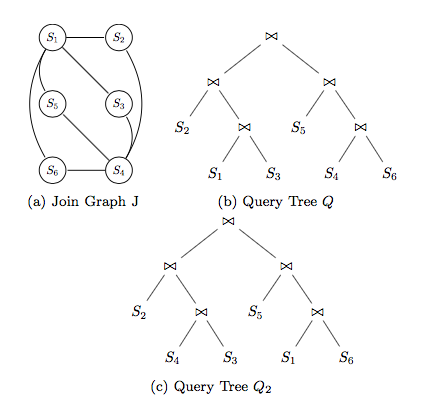
\includegraphics[width=\textwidth]{03_Related_Work/Incompleteness_RS-B2-CPS.png}
  \caption{Incompletness of RS-B2-CPS}
  \label{Incompleteness_RS-B2-CPS}
\end{figure}


\cite{shanbhag2014optimizing} stellt fest, dass RS-B0-CPS und RS-B1-CPS vollständig sind. Die Vollständigkeit von RS-B2-CPS wird jedoch in Frage gestellt und die Unvollständigkeit mit Hilfe eines Beispiels belegt. Als Beispiel dient eine Menge von Relationen, die mit Hilfe des Jointrees J (\ref{fig:Incompleteness_RS-B2-CPS}) miteinander gejoint sind. Der Initale Anfragebaum $Q1$ ist in \ref{fig:Incompleteness_RS-B2-CPS} dargestellt. Das gewünschte Ergebnis nach einer Transformation $Q2$  findet sich in \ref{fig:Incompleteness_RS-B2-CPS}. 

Bei RS-B2-CPS dürfen die Regeln R2, R3, R4 nur jeweils einmal auf einen Join-Operator angewendet werden. Keine der Regeln darf danach auf den neu generierten Operator angewendet werden. Die In \ref{fig:Q1} und \ref{fig:Q2} zeichnet sich dadurch aus, dass die Relationen $R1$ und $R4$ vertauscht sind.







\subsubsection{Vorschlag von RS-Graph}

\subsection{JOIN SETS}

Basierend auf dem bisherigen Wissen, wurden durch X und y einige neue Begriffe festgelegt:W
Ein Base Equivalence Knoten in einem expandierten LQDAG ist ein Äquivalenzknoten, der keinen Join Operator als Kinder hat. Ein solcher Knoten kann entweder eine Relation sein oder darf keine Join Operatoren als Kinder beinhalten.

Ein Join Tree ist in einem expandierten LQDAG ein Baum in der LQDAG dessen Wurzel ein Äuqivalenzknoten und jeder interne Knoten entweder ein Äquivalenzknoten oder ein Join Operator und jeder untergeordneter Knoten ein Äuqivalenzknoten ist.

Der Maximale JOIN Tree ist in einem expandierten LQDAG ein Join Tree, bei dem jeder Leaf knoten ein Base Equivalence Node ist.

Ein Join-Set für einen Äquivalenzknoten E ist in einem expandierten LQDAG ein Paar $J = (S, P)$ bei dem S ein Set von Äquivalenzknoten ist, deren 

\subsection{Ruleset RS-Graph}
Neben den bereits etablierten Regeln wird eine neue Regel für den Volcano Optimizer von \cite{shanbhag2014optimizing} vorgestellt. Die neue Transformationsregel $RS-Graph$ ersetzt die bisherigen Regeln und die bisherigen Regelsets. Die neue Regel erzeugt basierend auf einem Planknoten direkt alle möglichen äquivalenten Pläne. Somit sind alle Pläne unter einem bestimmten Äquivalenzknoten mit der Anwendung nur einer Regel erzeugt.

Die Regel $RS-Graph$ verwendet dazu die Subroutine $GraphRule$. Sie wird auf den Join Tree angewendet, falls die beiden mit einem Operator verbundenen Knoten A und B und deren Mitterknoten $P$. Für jedes Paar der J $$equivalence nodes A,B and parent equivalence node P. For each pair of join-set (jsA,jsB) ∈ A.JoinSets∗B.JoinSets, we merge the pair to form a join-set js. We define the merge of the two join-sets jsA = (V1,P1) and jsB = (V2,P2) as (V1∪V2,P1 ∧P2).$$

Um wiederholte Berechnungen des selben Join TRees zu vermeiden wird zudem geprüft, ob der Eltern-Äquivalenzknoten bereits $js$ beinhaltet. $$To check if two join- sets at an equivalence node are equal, it is sufficient to check if they have same equivalence nodes. If the join-sets have the same equivalence nodes, then they will also have the same predicates.$$

Für alle Join Sets $js$ des Parent nodes werden daraufhin zuerst alle JOIN partitionen gebildet bei denen $S_1 \Join S_2$ mit 

Sollte der $js$ noch nicht existieren, wird dieser dem JOIN Set hinzugefügt. Ein Graph wird basierend auf den $js$ gebildet, der mit Hilfe der Methode Partition in alle Partitionen getrennt wird. Aus denen wiederum Bäume erstellt werden, die an das Resultat zurückgegeben werden.

Die SubRoutine Create Graph, gibt ein JOIN Set, das JS einen Join Graphen aus, der




\subsection{Discussion}
Die Implementierung der neuen Regel wurde in einem Java basierten regelbasierten Optimierer implementiert. Dieser Optimierer “ProtoJ” ist eine Übersetzung des Optimierers Proto aus C++ in Java. Für die Implementierung mussten neue Felder den Äquivalenzklassen hinzugefügt werden.

Die Generierung der Resultate find ohne Pruning statt und kosten für die Kostenberechnung wurden nicht einbezogen. Ebenfalls bleiben Regeln bestehen, die für denn SELECT Pushdown verantwortlich sind, als teil der Normalisierungsphase. 

Es wurden sowohl Star, Chain als auch Clique Queries getestet. Die Experimente fanden auf einem Intel i5 3.5 GHz mit 8 GB Ram statt. Es wurde festgestellt, dass die Geschwindigkeit der Optimierung verbessert werden konnte, dadurch, dass die Optimierung mehrfach durchgeführt wurde. Dieses Verhalten wurde auf Javas JIT Kompilierungsstrategie zurückgeführt. Die erst den Code Kompiliert, wenn er auch tatsächlich gebraucht wird. Um sicherzustellen, dass der Kompilierte Code nicht wieder während der Ausführung vergessen geht mussten spezielle Flags für die JVM gesetzt werden. Das Ergebnis war, dass die Dauer zwar verglichen zu den schnellsten Test ohne das Flag langsamer, aber dafür konstant blieben.

Ebenfalls wurde bei Ruleset $RS_B1$ geprüft, ob der gesamte Search Space erreicht wurde, indem die Anzahl der Äquivalenten Knoten und Operatoren im LQDAG gezählt wurden. Diese Zahl wurde mit der Zahl der Knoten in RS-Graph verglichen. Da beide zahlen gleich war, wird davon ausgegangen, dass beide Regelsets das selbe Ergebnis erzeugen. Eine Prüfung, die dies belegt fand aus technischen Gründen nicht statt.






ersetzten X und Y die bisher gezeigten Regeln des Volcano Optimizers mit einer neuen Transformationsregel: RS-Graph. Die Regel kommt zur Anwendung, falls ein Graph dem Pattern $E_1 \Join E_2$ entspricht. Ist dies der Fall wird die Funktion $GraphRule(\Join, E_1, E_2, parent)$ aufgerufen. Sie erzeugt ein Set von allen Join Operatoren unter dem Equivalenzklasse des $parent$-Knotens.





